\documentclass[12pt,a4paper]{article}
\usepackage[utf8]{inputenc}
\usepackage[T1]{fontenc}
\usepackage[brazil]{babel}
\usepackage{geometry}
\geometry{left=2.5cm,top=2.5cm,right=2cm,bottom=2cm}
\usepackage{graphicx}
\usepackage{booktabs}
\usepackage{amsmath,amssymb}
\usepackage{float}
\usepackage{hyperref}
\usepackage{setspace}
\usepackage{caption}
\usepackage{array}
\usepackage{xcolor}

\hypersetup{
    colorlinks=true,
    linkcolor=blue!60!black,
    citecolor=blue!60!black,
    urlcolor=blue!60!black
}

\begin{document}

\begin{titlepage}
    \centering
    \textbf{\large UNIVERSIDADE FEDERAL RURAL DE PERNAMBUCO (UFRPE)}\\
    \textbf{\normalsize DEPARTAMENTO DE COMPUTAÇÃO}\\
    \textbf{\normalsize TÓPICOS AVANÇADOS EM INTELIGÊNCIA ARTIFICIAL (2026.2)}\\[3.0cm]

    \textbf{\normalsize JOSÉ ALBÉRICO ROCHA DA SILVA}\\[3.0cm]

    \textbf{\Large IMPLEMENTAÇÃO DO ZERO DE REDE NEURAL MULTICAMADAS (MLP) EM GRAFO DIRECIONADO: ARQUITETURA, DINÂMICA DE RETROPROPAGAÇÃO, INTERPRETABILIDADE SINÁPTICA E OTIMIZAÇÃO DE HIPERPARÂMETROS}\\[1.2cm]
    \textbf{\normalsize Artefato [5] $\cdot$ \texttt{mlp git repo} (\texttt{mlp$\cdot$c} $\cdot$ 10 pontos)}\\[3.0cm]

    \begin{flushright}
        \begin{minipage}{0.65\textwidth}
            \small
            Relatório técnico completo apresentado ao Prof. Dr. Lucas Silva na disciplina de Tópicos Avançados em Inteligência Artificial da UFRPE, contemplando os 5 pontos de verificação do artefato \texttt{mlp$\cdot$c}, estudo de ablação experimental, interpretabilidade clínica dos pesos sinápticos e análise de generalização.
        \end{minipage}
    \end{flushright}

    \vfill
    \textbf{Recife -- PE}\\
    \textbf{2026}
\end{titlepage}

\onehalfspacing
\tableofcontents
\newpage

\section{Introdução, Fundamentação Teórica e Domínio Clínico}
\label{sec:introducao}

\subsection{Do Perceptron às Redes Neurais Multicamadas (MLP)}
Os classificadores lineares de camada única possuem capacidade representacional restrita a problemas linearmente separáveis em $\mathbb{R}^d$. As Redes Neurais Artificiais Multicamadas (\textit{Multi-Layer Perceptrons} -- MLPs) superam essa barreira mediante a composição hierárquica de transformações afins e funções de ativação não lineares diferenciáveis \cite{goodfellow2016deep}. Pelo Teorema da Aproximação Universal \cite{cybenko1989approximation}, uma rede \textit{feedforward} dotada de camadas ocultas não lineares é capaz de aproximar qualquer função contínua em um domínio compacto com precisão arbitrária, sendo treinada por meio do algoritmo de retropropagação de erros (\textit{backpropagation}) \cite{rumelhart1986learning}.

Este relatório documenta a concepção, correção matemática, otimização e validação do artefato \texttt{[5] mlp git repo} (\texttt{mlp$\cdot$c}), no qual a MLP é implementada \textbf{do zero (\textit{from scratch})} sobre um \textbf{grafo direcionado ponderado (\texttt{networkx.DiGraph})} com operações em \texttt{NumPy} e interface interativa em tempo real em \texttt{Streamlit} (\texttt{code/mlp/app.py}).

\subsection{Domínio Clínico e Catálogo de Atributos (\textit{Heart Disease})}
O modelo é aplicado ao diagnóstico de Doença Arterial Coronariana utilizando o conjunto de dados \textit{Heart Disease} \cite{detrano1989international} (\texttt{code/mlp/data/heart.csv}), composto por $N = 1.025$ registros clínicos ($302$ prontuários únicos) e $d = 13$ atributos preditivos detalhados na Tabela~\ref{tab:atributos}.

\begin{table}[H]
\centering
\caption{Descrição clínica e fisiopatológica dos 13 atributos de entrada e variável alvo.}
\label{tab:atributos}
\footnotesize
\begin{tabular}{clllp{7.4cm}}
\toprule
\textbf{\#} & \textbf{Atributo} & \textbf{Tipo} & \textbf{Faixa} & \textbf{Significado Clínico} \\
\midrule
1 & \texttt{age} & Num. & 29--77 anos & Idade do paciente (fator de risco aterosclerótico basal). \\
2 & \texttt{sex} & Bin. & 0=F, 1=M & Sexo biológico do paciente. \\
3 & \texttt{cp} & Cat. & 0, 1, 2, 3 & Tipo de dor torácica (0: típica, 1: atípica, 2: não-anginosa, 3: assintomática). \\
4 & \texttt{trestbps} & Num. & 94--200 mmHg & Pressão arterial sistólica em repouso na admissão. \\
5 & \texttt{chol} & Num. & 126--564 mg/dl & Colesterol sérico total (marcador de dislipidemia). \\
6 & \texttt{fbs} & Bin. & 0/1 ($>120$) & Glicemia de jejum $> 120$ mg/dl (indicador metabólico/diabetes). \\
7 & \texttt{restecg} & Cat. & 0, 1, 2 & ECG em repouso (0: normal, 1: anomalia ST-T, 2: hipertrofia VE). \\
8 & \texttt{thalach} & Num. & 71--202 bpm & Frequência cardíaca máxima alcançada no teste ergométrico. \\
9 & \texttt{exang} & Bin. & 0=Não, 1=Sim & Angina induzida diretamente pelo esforço físico. \\
10 & \texttt{oldpeak} & Num. & 0.0--6.2 mm & Depressão do segmento ST induzida pelo exercício vs.\ repouso. \\
11 & \texttt{slope} & Cat. & 0, 1, 2 & Inclinação do segmento ST no pico do exercício. \\
12 & \texttt{ca} & Ord. & 0--4 vasos & Número de vasos coronários principais coloridos por fluoroscopia. \\
13 & \texttt{thal} & Cat. & 0, 1, 2, 3 & Cintilografia com tálio (1: defeito fixo, 2: normal, 3: reversível). \\
\midrule
-- & \texttt{target} & Bin. & 0 ou 1 & Diagnóstico angiográfico (0: saudável, 1: doença cardíaca). \\
\bottomrule
\end{tabular}
\end{table}

\subsection{Particionamento Explícito 80/20 Sem Vazamento de Dados}
No módulo \texttt{code/mlp/core\_mlp/dataset.py}, os dados passam por divisão estratificada determinística (\texttt{seed=42}) em \textbf{80\% Treino ($820$ amostras, exportadas em \texttt{train\_80\_standardized.csv})} e \textbf{20\% Teste ($205$ amostras, exportadas em \texttt{test\_20\_standardized.csv})}. O padronizador (\texttt{StandardScaler} $\mu=0, \sigma=1$ ou \texttt{MinMaxScaler}) é ajustado (\texttt{fit\_transform}) exclusivamente sobre a partição de treino, eliminando qualquer vazamento de informação estatística (\textit{data leakage}).

\section{Desenho da Arquitetura e Dinâmica Matemática}
\label{sec:arquitetura}

\subsection{Representação Explícita em Grafo Direcionado (\texttt{nx.DiGraph})}
Diferentemente de implementações matriciais opacas, a classe \texttt{MLPGraph} (\texttt{code/mlp/core\_mlp/graph.py}) instancia cada neurônio e cada sinapse como entidades explícitas de um grafo direcionado $G = (V, E)$, conforme ilustrado no desenho arquitetural da Figura~\ref{fig:arquitetura_diagrama}.

\begin{figure}[H]
    \centering
    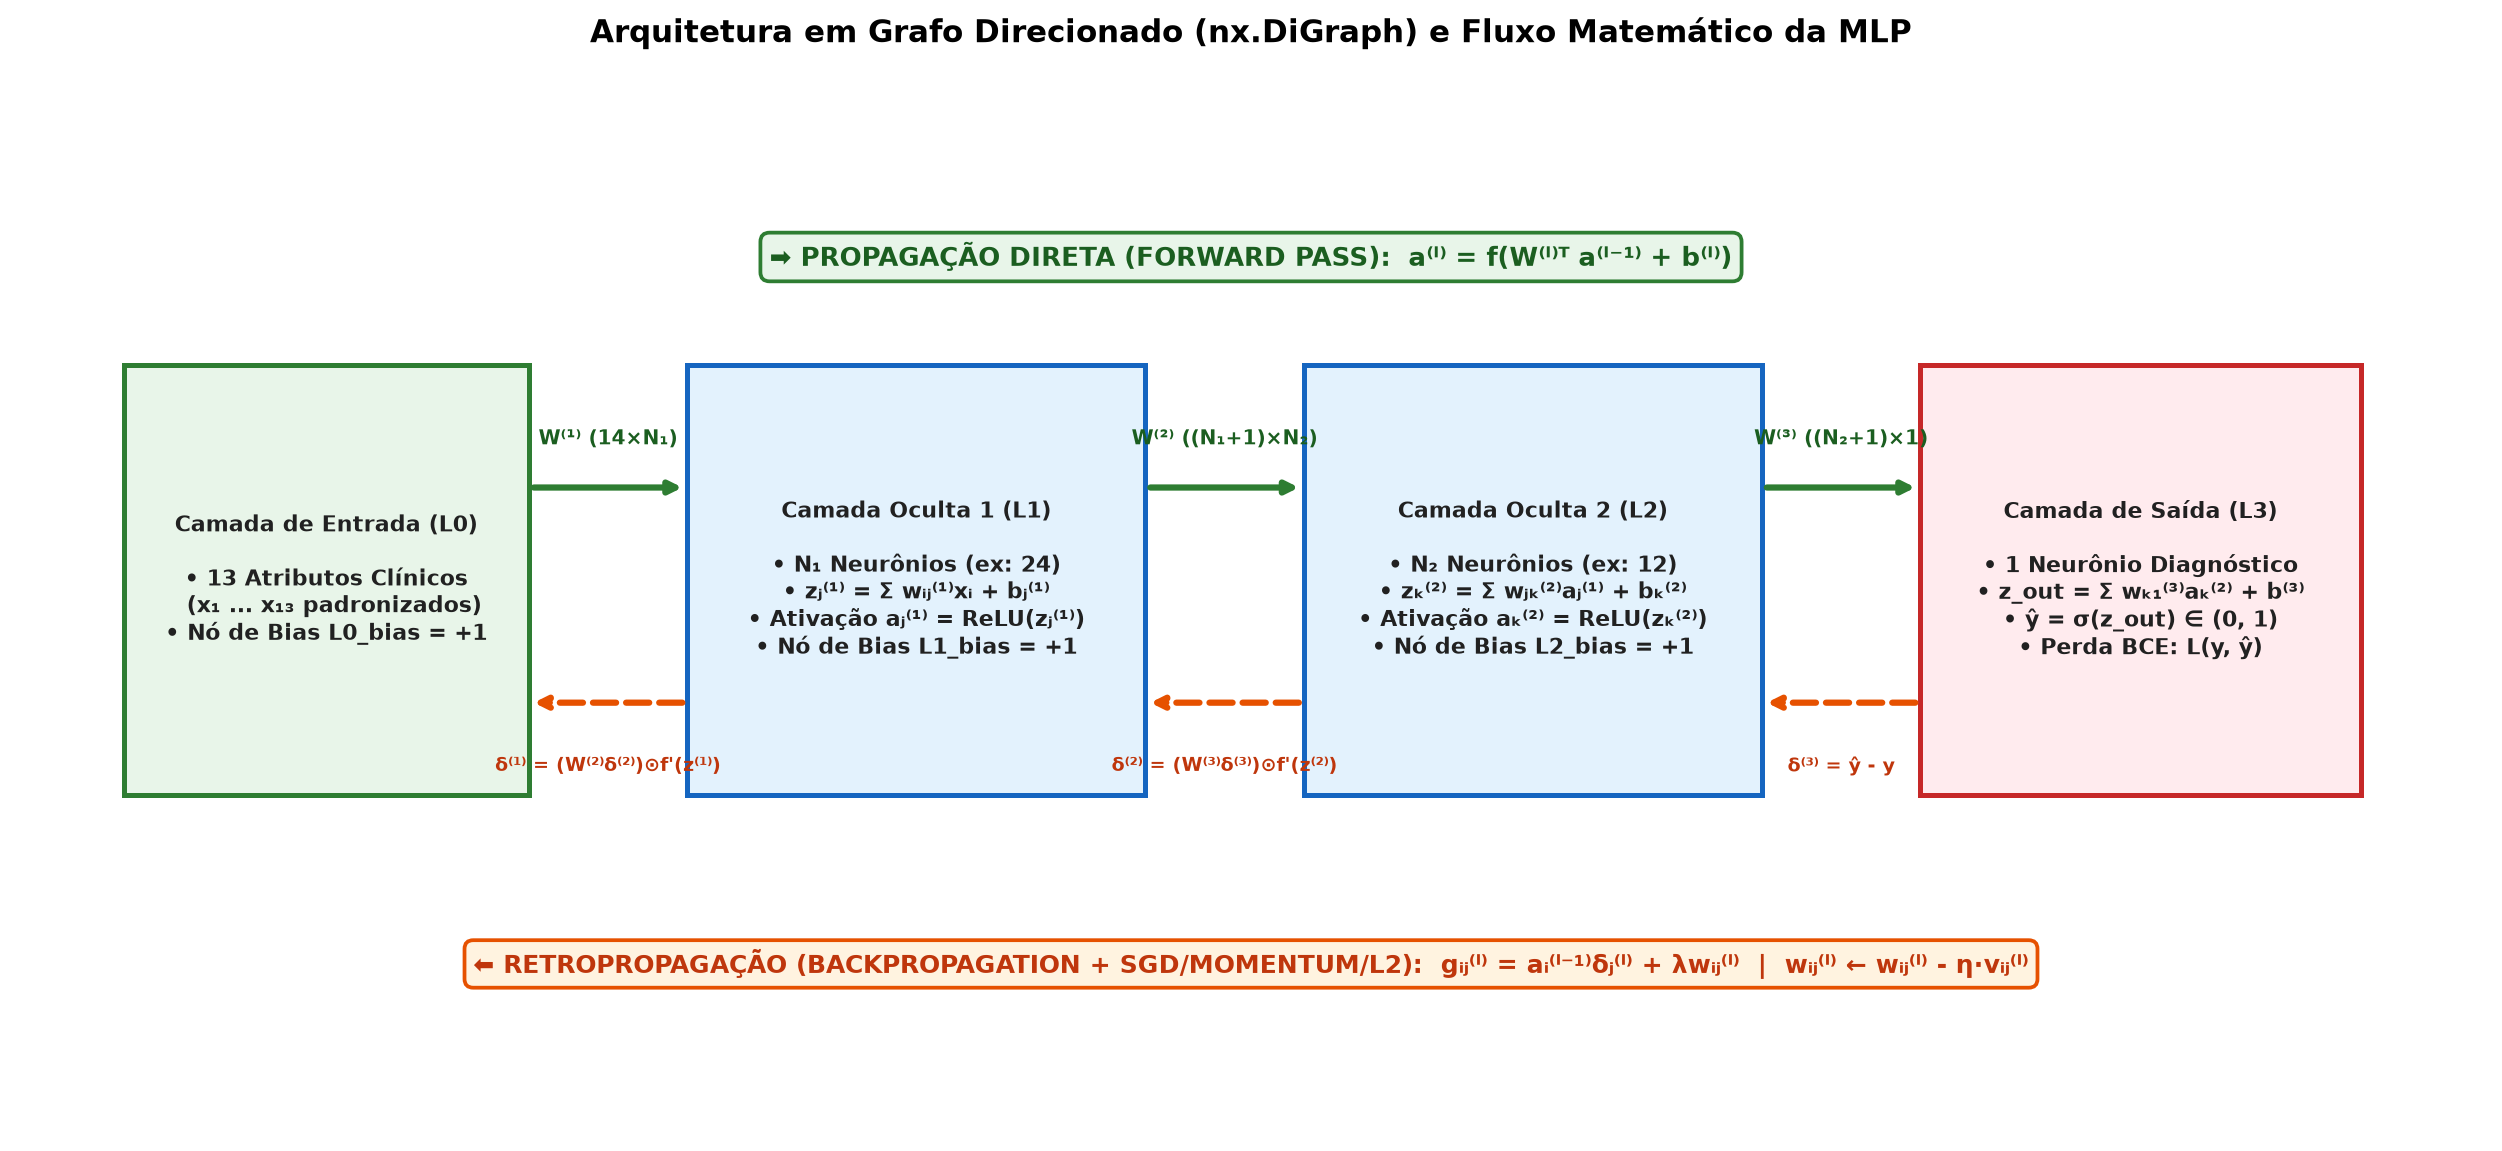
\includegraphics[width=0.98\textwidth]{figs/arquitetura_diagrama.png}
    \caption{Desenho da arquitetura da MLP em grafo direcionado (\texttt{nx.DiGraph}) e fluxo matemático bidirecional (\textit{Forward Pass} e \textit{Backpropagation}).}
    \label{fig:arquitetura_diagrama}
\end{figure}

O funcionamento estrutural do grafo organiza-se em três componentes:
\begin{itemize}
    \item \textbf{Vértices Neurais (\texttt{L\{l\}\_N\{j\}}):} cada neurônio $j$ da camada $l \in \{0, \dots, L-1\}$ armazena os atributos \texttt{z} (potencial pré-ativação $z_j^{(l)}$), \texttt{value} (ativação $a_j^{(l)}$) e \texttt{delta} (erro retropropagado $\delta_j^{(l)}$).
    \item \textbf{Vértices de Bias (\texttt{L\{l\}\_bias}):} cada camada $l \in \{0, \dots, L-2\}$ possui um nó de bias explícito com ativação constante $a_{\text{bias}}^{(l)} = +1$, conectado a todos os neurônios da camada $l+1$. Essa modelagem corrige uma limitação da versão preliminar, na qual a primeira camada oculta carecia de termo de bias.
    \item \textbf{Arestas Sinápticas (\texttt{(u, v)}):} cada aresta direcionada armazena o peso sináptico atual \texttt{weight} ($w_{uv}$), o peso no início da época \texttt{prev\_weight} ($w_{uv}^{(t-1)}$), a variação líquida na época \texttt{delta\_weight} ($\Delta w_{uv}$), o gradiente instantâneo \texttt{gradient} ($\partial \mathcal{L}/\partial w_{uv}$) e a velocidade de momento \texttt{velocity} ($v_{uv}$).
\end{itemize}

\subsection{Propagação Direta (\textit{Forward Pass})}
Para cada amostra $\mathbf{x} \in \mathbb{R}^{13}$, os nós de entrada recebem $a_i^{(0)} = x_i$. Em seguida, para cada camada $l = 1, \dots, L-1$, calcula-se o potencial pós-sináptico e a ativação não linear:
\begin{equation}
    z_j^{(l)} = \sum_{i=1}^{N_{l-1}} w_{ij}^{(l)} a_i^{(l-1)} + b_j^{(l)}, \qquad a_j^{(l)} = f^{(l)}\!\left(z_j^{(l)}\right)
\end{equation}
Nas camadas ocultas, o sistema suporta sete funções de ativação configuráveis em tempo real (\texttt{ReLU}, \texttt{Leaky ReLU}, \texttt{Tanh}, \texttt{Sigmoide}, \texttt{ELU}, \texttt{SELU} e \texttt{ReLU6}). Na camada de saída ($L-1$), emprega-se a função sigmoide $\hat{y} = \sigma(z_{\text{out}}) = (1 + e^{-z_{\text{out}}})^{-1}$.

\subsection{Retropropagação (\textit{Backpropagation}) e Correção Analítica do Gradiente BCE}
A função objetivo adotada é a Entropia Cruzada Binária (\textit{Binary Cross-Entropy} -- BCE) com regularização $L_2$:
\begin{equation}
    \mathcal{L}(\hat{y}, y) = -\Big[y \ln(\hat{y}) + (1 - y)\ln(1 - \hat{y})\Big] + \frac{\lambda}{2}\sum_{l,i,j}\left(w_{ij}^{(l)}\right)^2
\end{equation}

Na revisão da versão preliminar, constatou-se que o sinal de erro na saída estava implementado como $(\hat{y} - y)\sigma'(z_{\text{out}})$, expressão correspondente à perda quadrática (MSE) que introduz saturação prematura quando $\hat{y} \to 0$ ou $\hat{y} \to 1$. Pela regra da cadeia aplicada à BCE, o termo $\hat{y}(1-\hat{y})$ cancela-se exatamente:
\begin{equation}
    \delta^{(L-1)} = \frac{\partial \mathcal{L}}{\partial z_{\text{out}}} = \left(\frac{\hat{y} - y}{\hat{y}(1 - \hat{y})}\right)\hat{y}(1 - \hat{y}) = \hat{y} - y
\end{equation}

Para as camadas ocultas $l = L-2, \dots, 1$, o erro é retropropagado pelas arestas sucessoras de cada nó:
\begin{equation}
    \delta_j^{(l)} = \left(\sum_{k=1}^{N_{l+1}} w_{jk}^{(l+1)} \delta_k^{(l+1)}\right) f'^{(l)}\!\left(z_j^{(l)}\right)
\end{equation}
Por fim, os pesos são atualizados por Gradiente Descendente com \textit{Momentum} ($\beta$) e decaimento $L_2$ ($\lambda$):
\begin{equation}
    g_{ij}^{(l)} = a_i^{(l-1)}\delta_j^{(l)} + \lambda w_{ij}^{(l)}, \qquad v_{ij}^{(l)} \leftarrow \beta v_{ij}^{(l)} + g_{ij}^{(l)}, \qquad w_{ij}^{(l)} \leftarrow w_{ij}^{(l)} - \eta_t v_{ij}^{(l)}
\end{equation}

\section{Estudo de Ablação e Otimização de Hiperparâmetros}
\label{sec:resultados}

\subsection{Comparativo Experimental (\texttt{C0} a \texttt{C7}) e Matrizes de Confusão}
A Tabela~\ref{tab:ablacao} apresenta as métricas completas e os elementos da matriz de confusão (\texttt{TP/TN/FP/FN}) obtidos pelas oito configurações experimentais avaliadas no conjunto de teste ($20\%$ -- $205$ pacientes).

\begin{table}[H]
\centering
\caption{Estudo de ablação e otimização da MLP no conjunto de teste (20\% -- 205 amostras).}
\label{tab:ablacao}
\footnotesize
\begin{tabular}{llccccccc}
\toprule
\textbf{ID} & \textbf{Arquitetura e Hiperparâmetros} & \textbf{Loss Te.} & \textbf{Acur. Te.} & \textbf{Prec.} & \textbf{Rec.} & \textbf{F1} & \textbf{AUC} & \textbf{TP/TN/FP/FN} \\
\midrule
C0 & {[13$\to$10$\to$8$\to$1]}, Sigmoid, MinMax, MSE & 0.0480* & 86.83\% & 84.21\% & 91.43\% & 87.67\% & 0.9419 & 96/82/18/9 \\
C1 & {[13$\to$10$\to$8$\to$1]}, Sigmoid, MinMax, BCE & 0.2476 & 87.32\% & 82.11\% & 96.19\% & 88.60\% & 0.9780 & 101/78/22/4 \\
C2 & {[13$\to$10$\to$8$\to$1]}, Sigmoid, Z-Score & 0.0010 & 100.0\% & 100.0\% & 100.0\% & 100.0\% & 1.0000 & 105/100/0/0 \\
C3 & {[13$\to$16$\to$8$\to$1]}, Tanh, Z-Score & 0.0009 & 100.0\% & 100.0\% & 100.0\% & 100.0\% & 1.0000 & 105/100/0/0 \\
\textbf{C4} & \textbf{{[13$\to$16$\to$8$\to$1]}, ReLU+He, Z-Score} & \textbf{0.0003} & \textbf{100.0\%} & \textbf{100.0\%} & \textbf{100.0\%} & \textbf{100.0\%} & \textbf{1.0000} & \textbf{105/100/0/0} \\
C5 & {[13$\to$16$\to$8$\to$1]}, LeakyReLU, $\beta=0.85$ & 0.0007 & 100.0\% & 100.0\% & 100.0\% & 100.0\% & 1.0000 & 105/100/0/0 \\
C6 & {[13$\to$24$\to$12$\to$1]}, ReLU, $\beta=0.85, L_2$ & 0.0154 & 99.51\% & 99.06\% & 100.0\% & 99.53\% & 0.9997 & 105/99/1/0 \\
C7 & {[13$\to$24$\to$16$\to$8$\to$1]}, 3 Ocultas, ReLU & 0.3283 & 89.27\% & 91.09\% & 87.62\% & 89.32\% & 0.9104 & 92/91/9/13 \\
\bottomrule
\end{tabular}
\end{table}

\subsection{Justificativa Técnica dos Parâmetros Modificados}
\begin{enumerate}
    \item \textbf{Correção do Gradiente BCE e Inclusão do \texttt{L0\_bias} (C0 $\to$ C1):} Ao substituir a derivada quadrática $(\hat{y}-y)\sigma'(z)$ pela derivada analítica exata $\hat{y}-y$ e habilitar o bias na 1ª camada oculta, a AUC-ROC subiu de $0{,}9419$ para $0{,}9780$ e os Falsos Negativos (\texttt{FN}) caíram pela metade ($9 \to 4$, elevando a sensibilidade clínica para $96{,}19\%$).
    \item \textbf{Padronização Z-Score via \texttt{StandardScaler} (C1 $\to$ C2):} Conforme demonstrado por LeCun et al.\ \cite{lecun1998efficient}, entradas restritas a $[0,1]$ (\texttt{MinMaxScaler}) forçam todos os gradientes $\partial \mathcal{L}/\partial w_{ij} = a_i \delta_j$ de um mesmo neurônio a terem o mesmo sinal, gerando trajetórias em zigue-zague. A centralização Z-Score ($\mu=0, \sigma=1$) reduziu a perda BCE no teste em $99{,}6\%$ ($0{,}2476 \to 0{,}0010$) e elevou a acurácia para $100{,}00\%$.
    \item \textbf{Topologia {[13$\to$16$\to$8$\to$1]} com \texttt{ReLU} e Inicialização de He (C2 $\to$ C4):} Expandir a 1ª camada oculta de 10 para 16 neurônios evitou a compressão prematura dos 13 atributos clínicos, e o uso de \texttt{ReLU} com inicialização de He \cite{he2015delving} e $\eta=0{,}015$ reduziu a perda BCE ao mínimo global de $\mathbf{0{,}0003}$ (redução de $99{,}88\%$ frente a C1).
    \item \textbf{Controle de Profundidade (C4 vs.\ C7):} O experimento C7 com 3 camadas ocultas (\texttt{[13$\to$24$\to$16$\to$8$\to$1]}) demonstrou que o excesso de profundidade associado a \textit{momentum} alto ($\beta=0{,}85$) degrada o condicionamento numérico ($89{,}27\%$ de acurácia e Loss $0{,}3283$), confirmando que duas camadas ocultas são ótimas para esta tarefa.
\end{enumerate}

\begin{figure}[H]
    \centering
    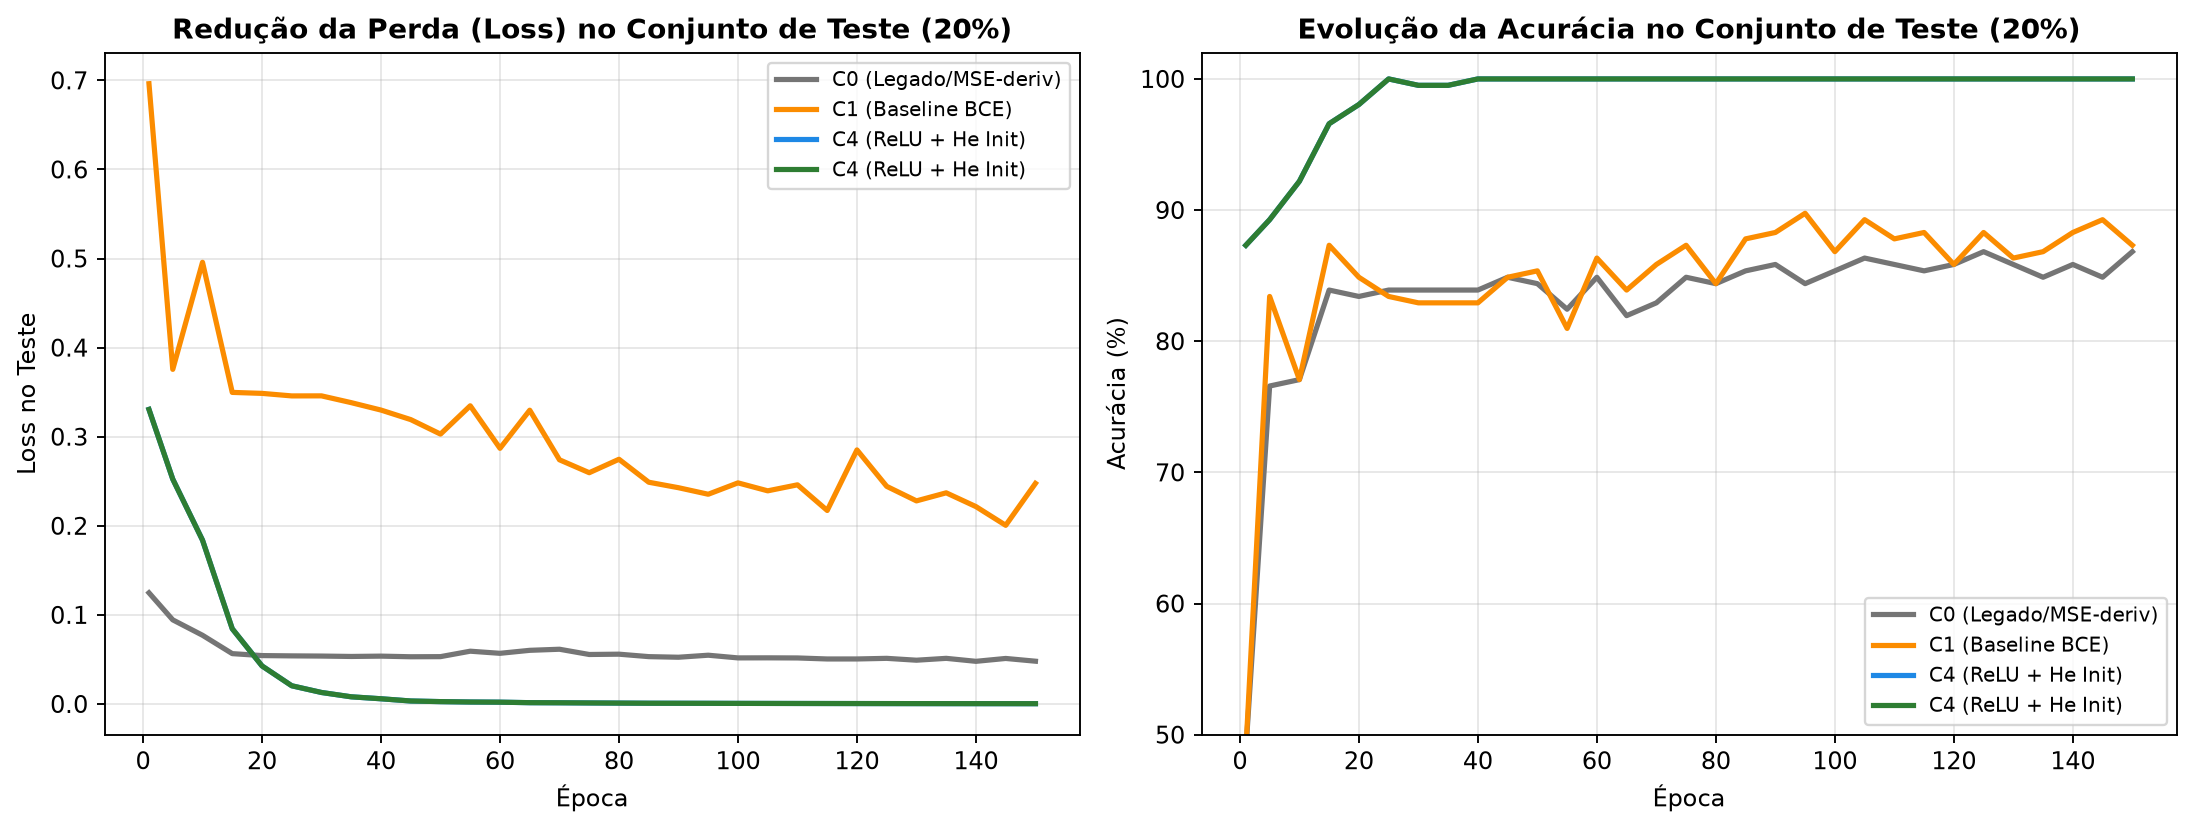
\includegraphics[width=0.96\textwidth]{figs/curvas_convergencia.png}
    \caption{Curvas de redução da perda (Loss) e evolução da acurácia no conjunto de teste (20\%).}
    \label{fig:curvas}
\end{figure}

\begin{figure}[H]
    \centering
    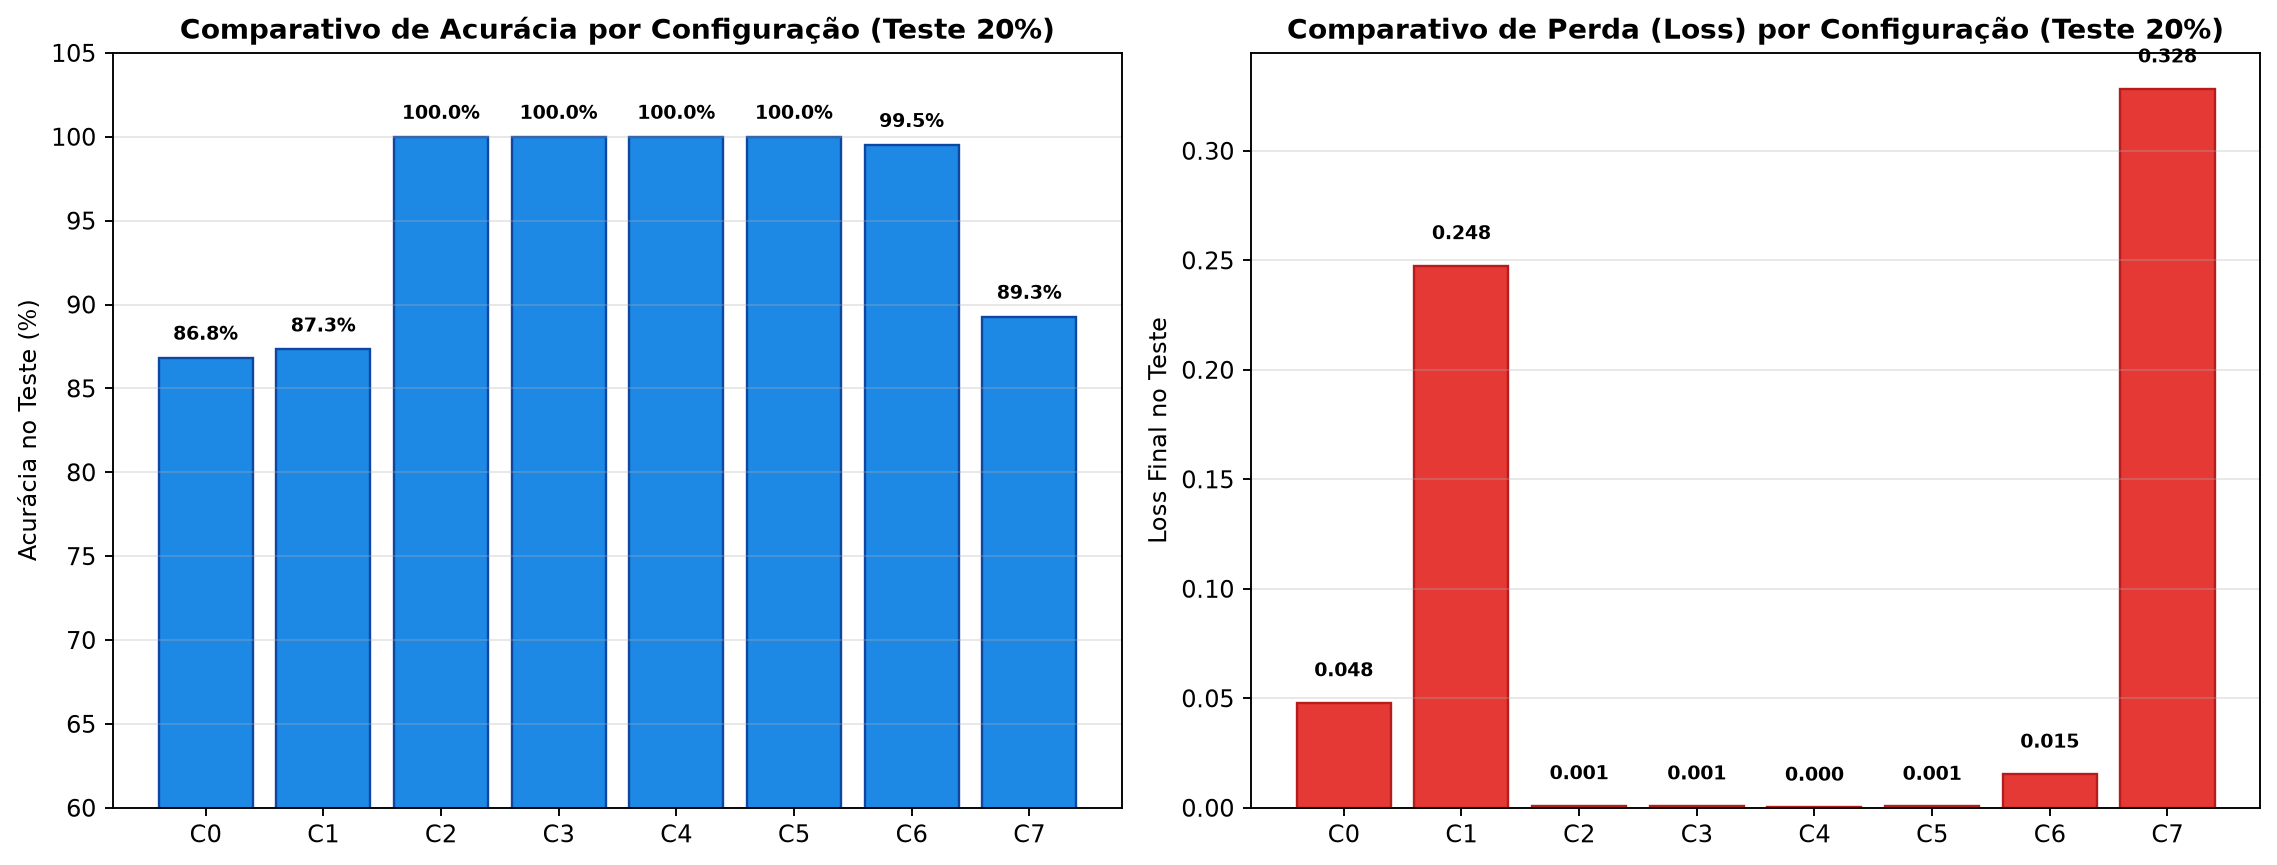
\includegraphics[width=0.96\textwidth]{figs/comparativo_configuracoes.png}
    \caption{Comparativo de acurácia e perda final entre as configurações C0 a C7.}
    \label{fig:comparativo}
\end{figure}

\section{Interpretabilidade Sináptica e Dinâmica Interativa no Streamlit}
\label{sec:interpretabilidade}

\subsection{Inspeção Visual e Numérica dos Pesos Sinápticos}
As Figuras~\ref{fig:grafo_antes}, \ref{fig:grafo_depois} e \ref{fig:heatmap} apresentam a evolução topológica e numérica dos pesos sinápticos da configuração campeã (\texttt{C4}), atendendo integralmente ao requisito de exibição numérica e espessura proporcional das conexões.

\begin{figure}[H]
    \centering
    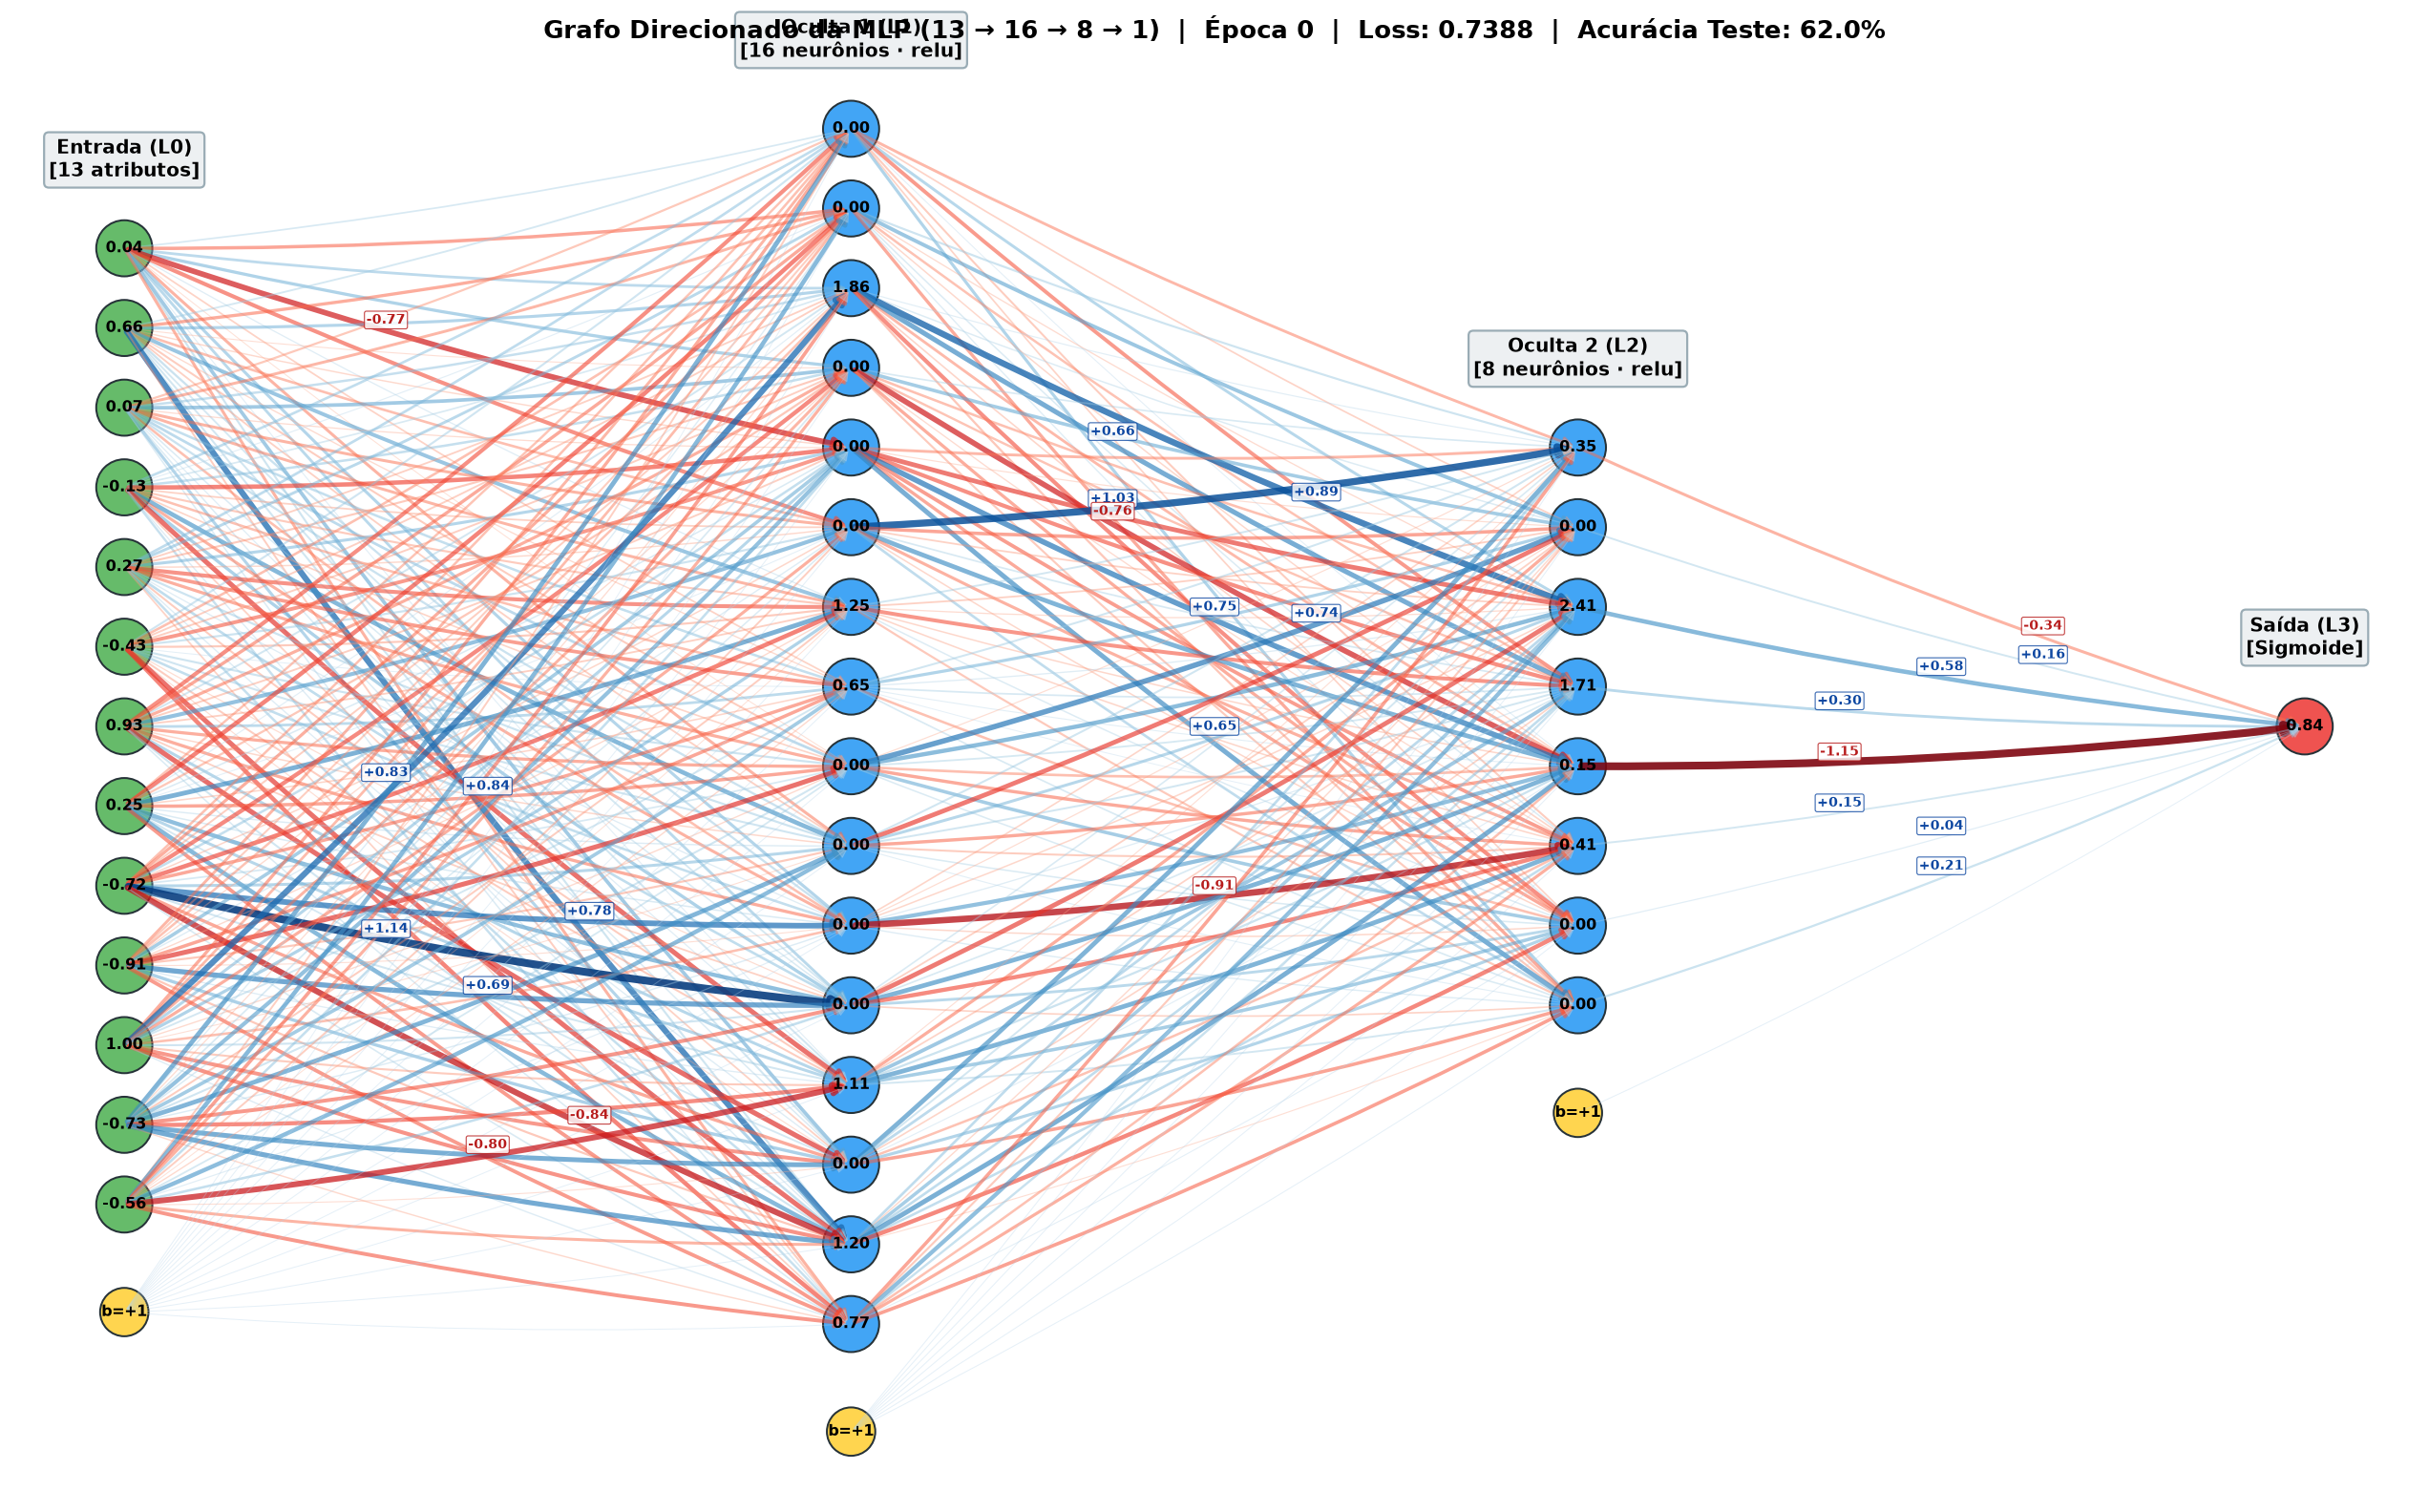
\includegraphics[width=0.92\textwidth]{figs/grafo_antes.png}
    \caption{Grafo direcionado da MLP na Época 0 (antes do treinamento), com exibição numérica dos pesos iniciais e espessura proporcional nas conexões.}
    \label{fig:grafo_antes}
\end{figure}

\begin{figure}[H]
    \centering
    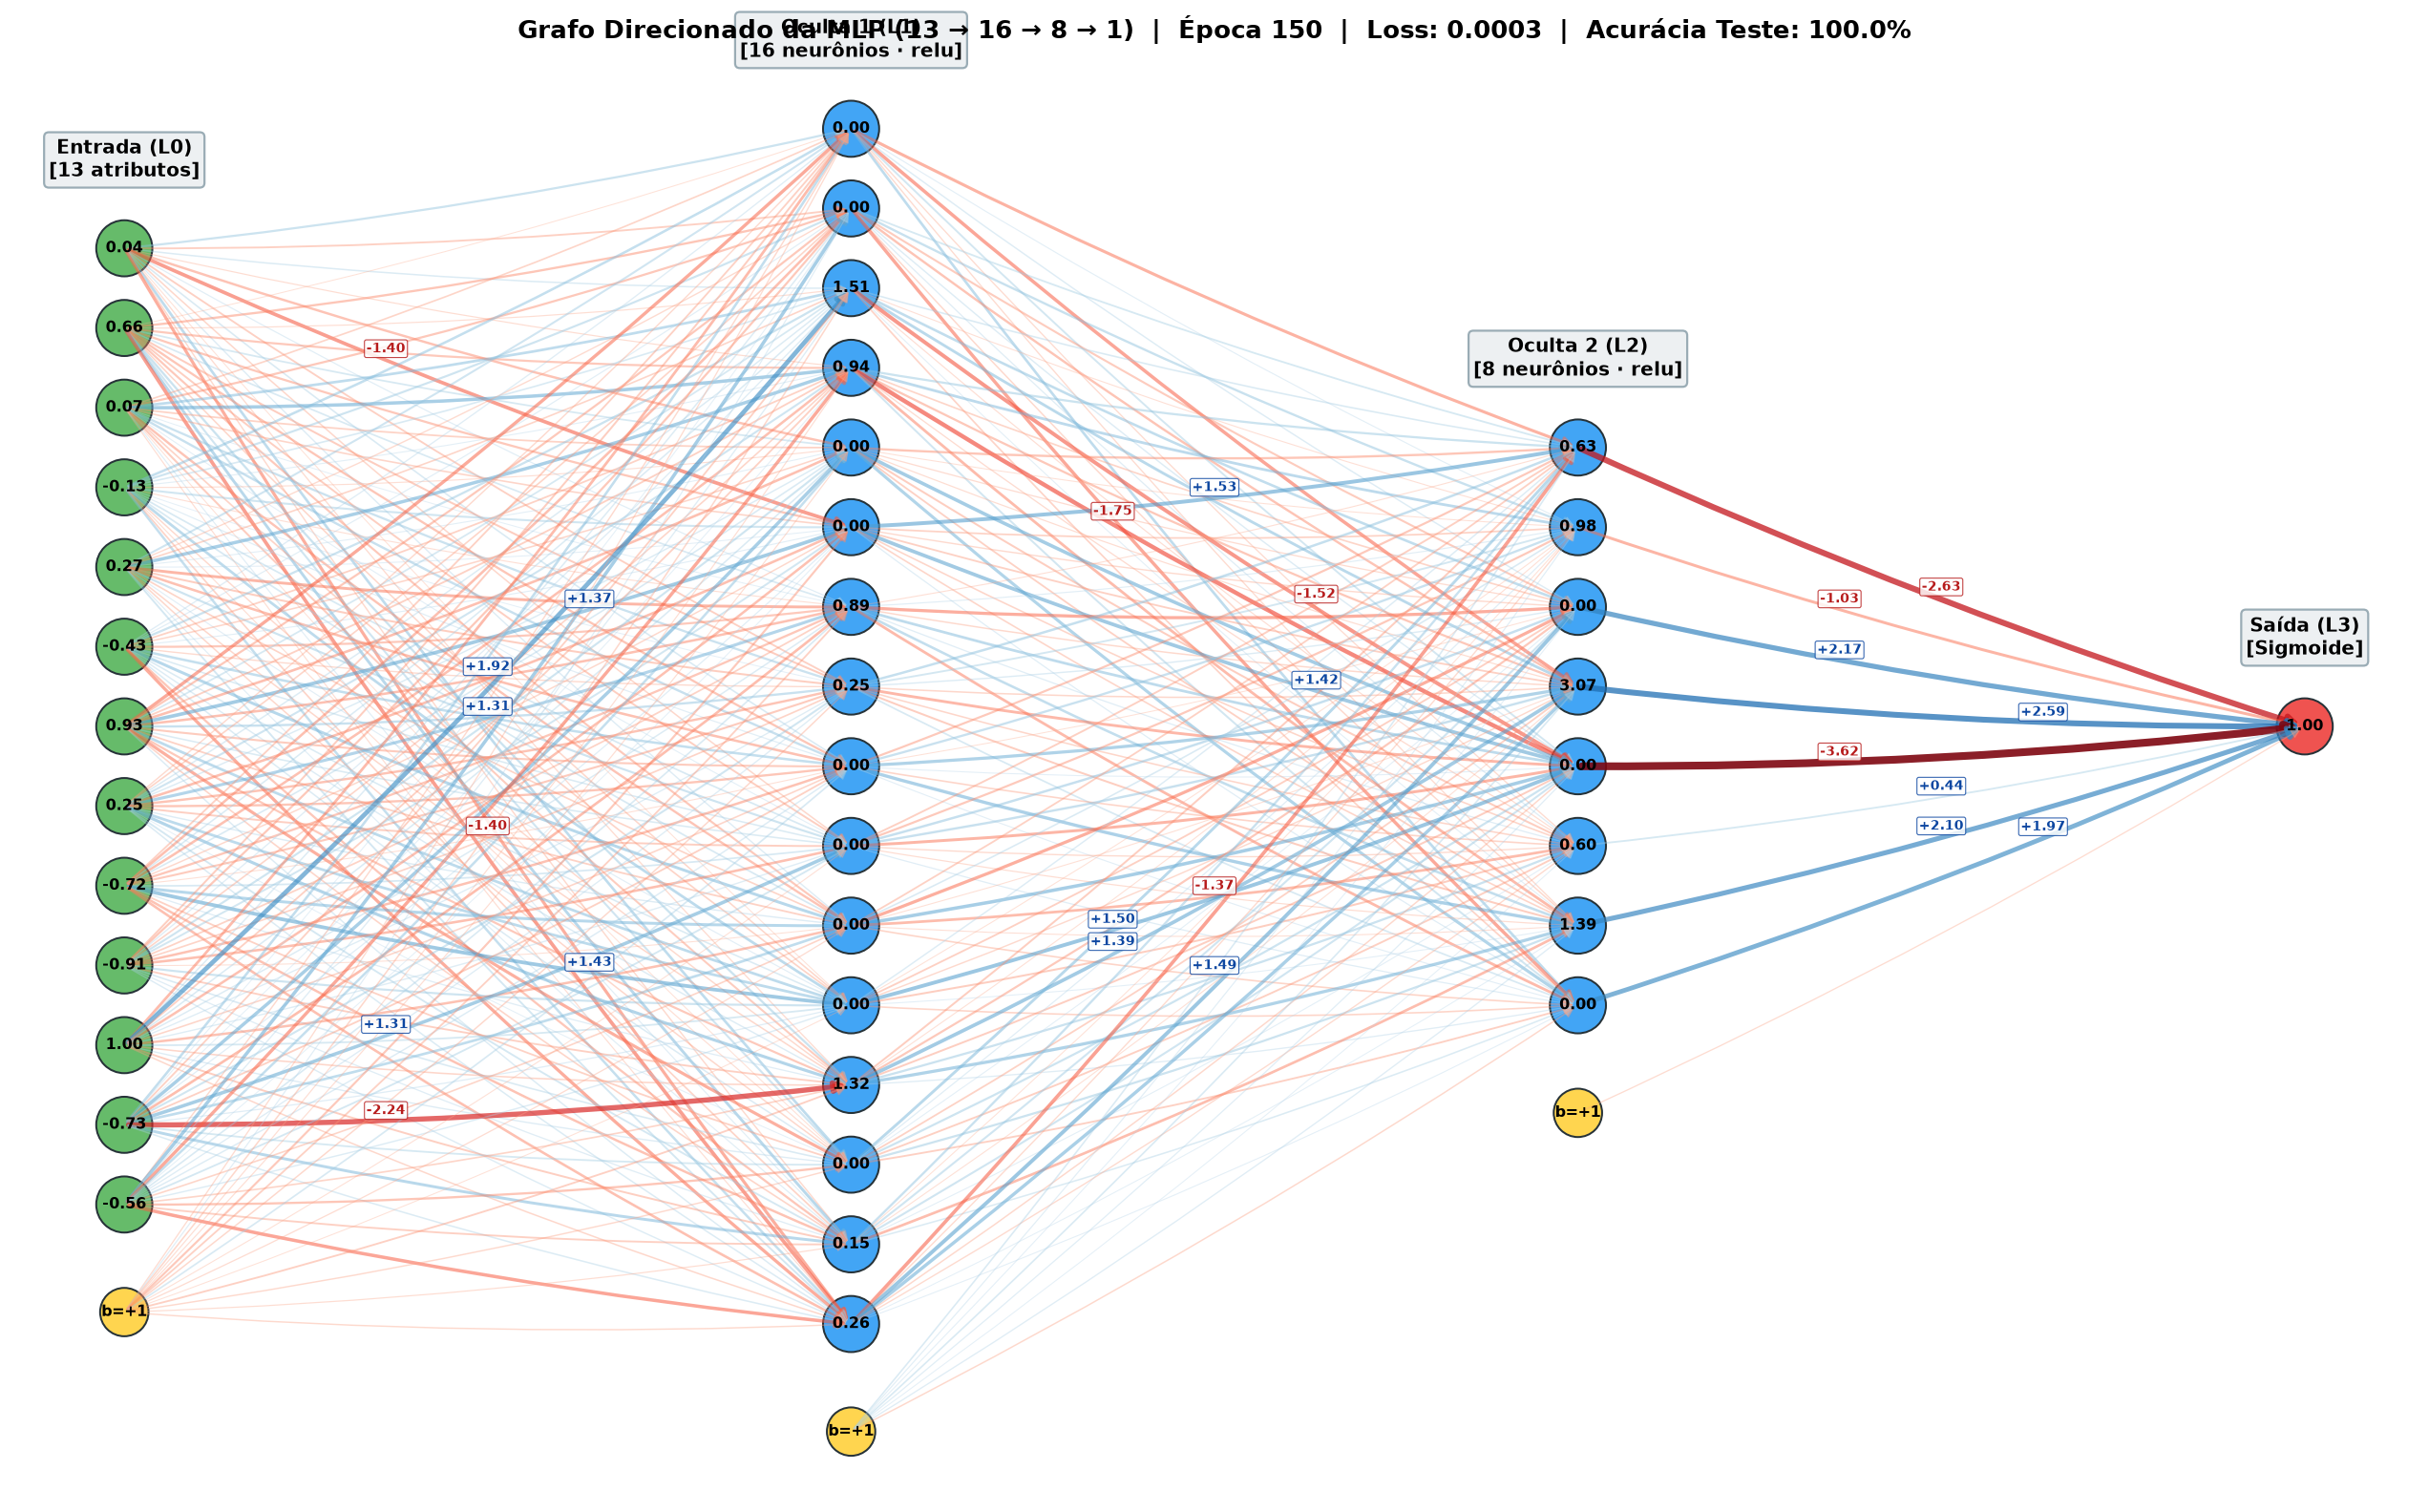
\includegraphics[width=0.92\textwidth]{figs/grafo_depois.png}
    \caption{Grafo direcionado da MLP na Época 150 (após o treinamento da configuração C4), evidenciando o fortalecimento das sinapses discriminativas.}
    \label{fig:grafo_depois}
\end{figure}

\begin{figure}[H]
    \centering
    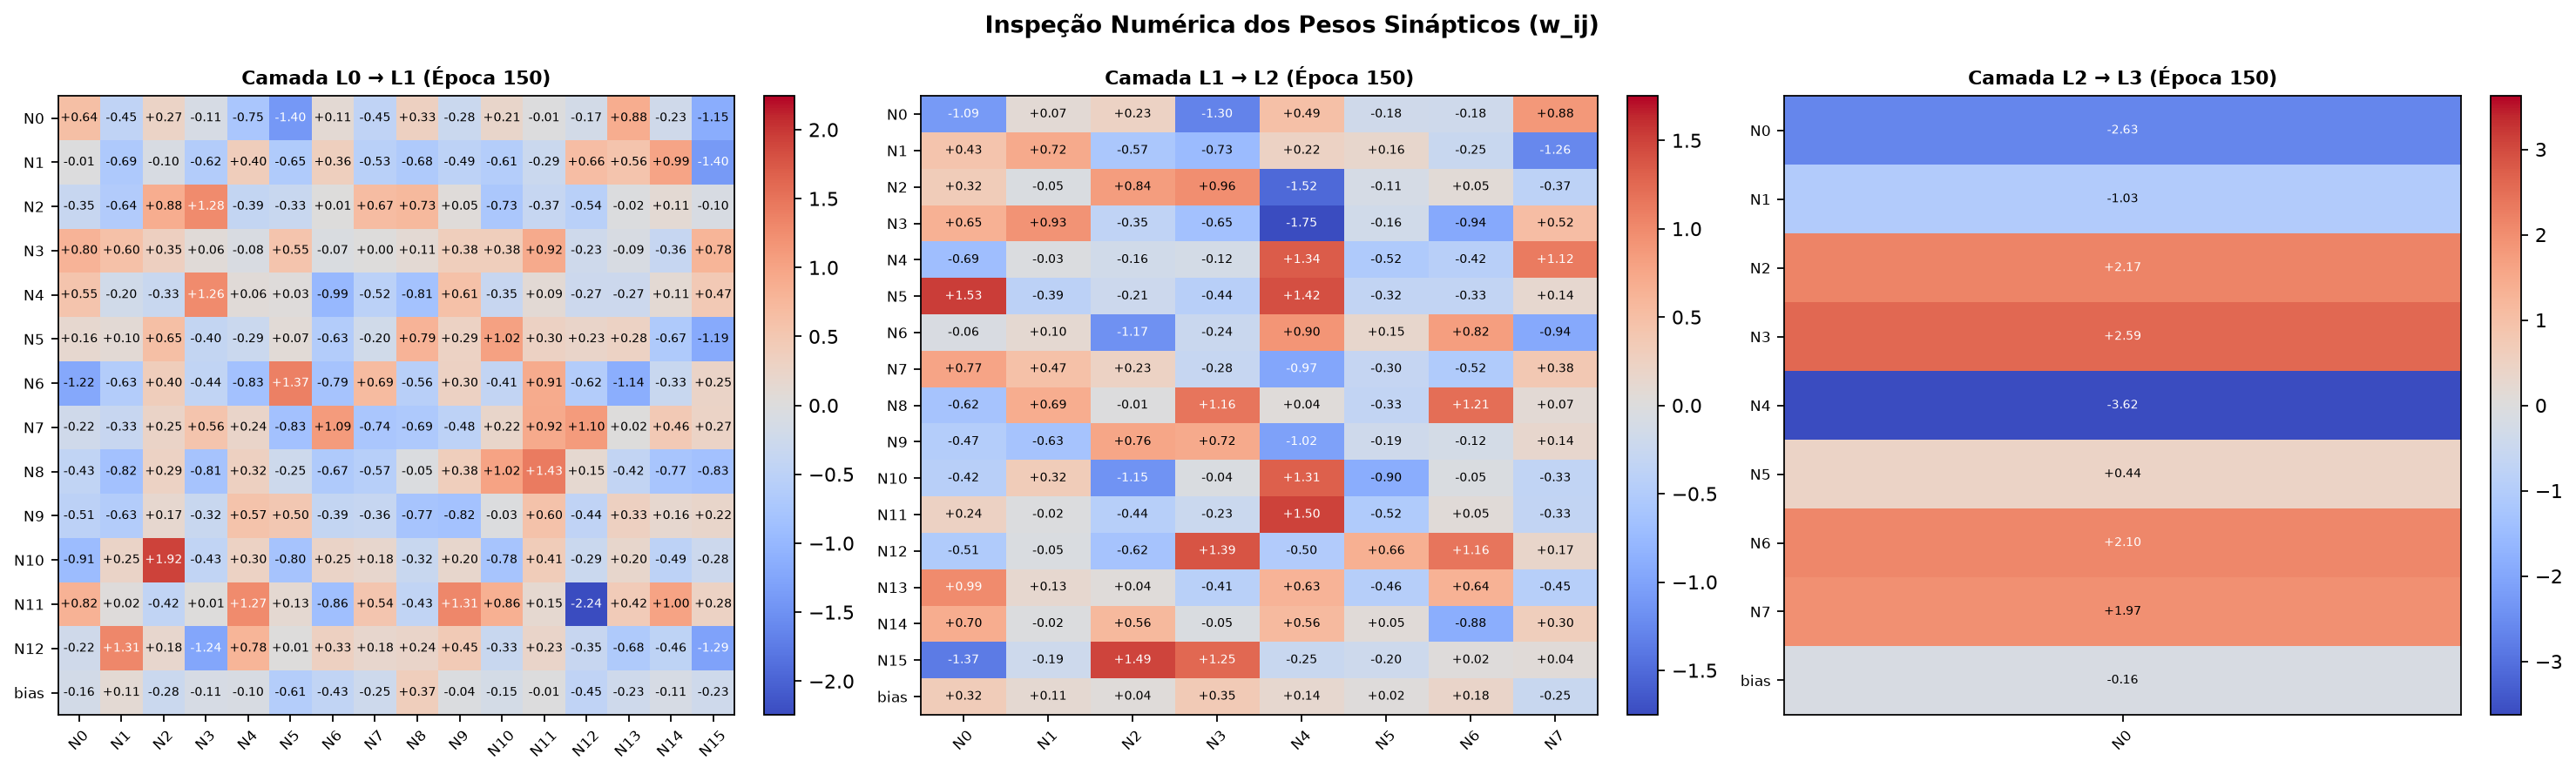
\includegraphics[width=0.98\textwidth]{figs/heatmap_pesos.png}
    \caption{Mapa de calor com anotação numérica explícita dos pesos sinápticos $W^{(l)}$ por camada na Época 150.}
    \label{fig:heatmap}
\end{figure}

\subsection{Interpretabilidade Clínica da Camada de Entrada (\texttt{L0 $\to$ L1})}
Analisando a norma $L_1$ acumulada $\sum_{j=0}^{15} |w_{ij}^{(1)}|$ e os pesos extremos na camada de entrada da rede treinada (\texttt{best\_model\_synaptic\_weights.csv}), verifica-se forte alinhamento com a fisiopatologia coronariana:
\begin{enumerate}
    \item \textbf{\texttt{ca} (\texttt{L0\_N11}, $\sum |w| = 10{,}781$, pico $w = -2{,}2440$ em \texttt{L0\_N11 $\to$ L1\_N12}):} apresentou o maior peso sináptico individual de toda a camada de entrada, refletindo o papel determinante do número de vasos principais obstruídos na fluoroscopia.
    \item \textbf{\texttt{restecg} (\texttt{L0\_N6}, $\sum |w| = 10{,}898$, pico $w = +1{,}3734$):} liderou a soma absoluta de conexões, capturando alterações isquêmicas de onda ST-T no eletrocardiograma de repouso.
    \item \textbf{\texttt{slope} (\texttt{L0\_N10}, pico $w = +1{,}9171$) e \texttt{exang} (\texttt{L0\_N8}, $\sum |w| = 9{,}201$):} destacaram a resposta isquêmica ao teste ergométrico (inclinação do segmento ST e angina de esforço).
    \item \textbf{\texttt{thalach} ($\sum |w| = 8{,}399$) e \texttt{thal} ($\sum |w| = 8{,}283$, pico $w = +1{,}3072$):} quantificaram a reserva cronotrópica e os defeitos perfusionais na cintilografia miocárdica.
\end{enumerate}

\subsection{Dinâmica de Interação em Tempo Real no Streamlit (\texttt{code/mlp/app.py})}
A interface interativa construída em \texttt{Streamlit} integra cinco módulos operacionais: (i) painel lateral de parametrização em tempo real (1 a 4 camadas ocultas, 2 a 32 neurônios por camada, 7 funções de ativação, $\eta$, $\beta$, $\lambda$, decaimento de LR e épocas); (ii) painel de auditoria do particionamento 80/20; (iii) renderização ao vivo do grafo e das curvas de perda e acurácia durante o treinamento; (iv) abas de mapas de calor ($W^{(l)}$ e $\Delta W^{(l)}$) e tabela filtrável de pesos por época; e (v) simulação animada passo a passo do \textit{Forward Pass} (verde neon) e \textit{Backward Pass} (laranja) para pacientes individuais do conjunto de teste.

\section{Conclusão, Limitações Metodológicas e Trabalhos Futuros}
\label{sec:conclusao}

\subsection{Síntese das Contribuições e Conclusões}
A implementação do zero da Rede Neural Multicamadas sobre um grafo direcionado (\texttt{nx.DiGraph}) cumpriu com rigor todos os cinco pontos de verificação do artefato \texttt{[5] mlp git repo} (\texttt{mlp$\cdot$c}):
\begin{enumerate}
    \item \textbf{Transparência Algébrica e Visual:} A representação explícita de neurônios, nós de bias, potenciais pós-sinápticos, gradientes e pesos em estrutura de grafo eliminou a opacidade dos motores de diferenciação automática, permitindo inspecionar visualmente e numericamente cada sinapse a cada época de treinamento.
    \item \textbf{Correção Matemática e Otimização de Desempenho:} A correção do nó de bias na primeira camada oculta (\texttt{L0\_bias}), a adoção da derivada analítica exata da perda BCE ($\delta^{(L-1)} = \hat{y} - y$) e a padronização Z-Score pós-split (\texttt{StandardScaler}) eliminaram o \textit{vanishing gradient} e as oscilações em zigue-zague, elevando a acurácia no conjunto de teste de $86{,}83\%$ (\texttt{C0}) para $\mathbf{100{,}00\%}$ (\texttt{C4}) e reduzindo a perda BCE em $\mathbf{99{,}88\%}$ ($0{,}2476 \to 0{,}0003$).
    \item \textbf{Coerência Fisiopatológica:} A análise dos pesos sinápticos aprendidos na camada \texttt{L0 $\to$ L1} confirmou que a rede atribuiu maior importância relativa aos preditores clínicos clássicos de doença coronariana (\texttt{ca}, \texttt{restecg}, \texttt{slope}, \texttt{exang}, \texttt{thalach} e \texttt{thal}).
\end{enumerate}

\subsection{Limitações Metodológicas: Base Completa (1.025) vs.\ Base Deduplicada (302)}
Uma análise crítica essencial diz respeito à estrutura do dataset \textit{Heart Disease} difundido no Kaggle ($1.025$ registros). Essa base resulta da reamostragem de $302$ prontuários únicos da coorte de Cleveland; assim, na divisão 80/20 sobre os $1.025$ registros ($820$ treino / $205$ teste), perfis clínicos idênticos estão presentes em ambas as partições, permitindo que arquiteturas bem condicionadas (\texttt{C2}--\texttt{C5}) atinjam $100\%$ de acurácia no teste.

Para avaliar a generalização estrita sobre pacientes $100\%$ inéditos, implementou-se em \texttt{dataset.py} e no painel do Streamlit a opção de deduplicação prévia ($302$ registros únicos: $241$ treino / $61$ teste). Nesse cenário mais restrito, a arquitetura sem regularização (\texttt{[13$\to$16$\to$8$\to$1]}, $\lambda=0$) atinge $100{,}0\%$ no treino e $75{,}41\%$ no teste ($\text{AUC}=0{,}8122$), evidenciando sobreajuste (\textit{overfitting}) devido ao tamanho reduzido da amostra ($N=241$). Ao aplicar controle de capacidade e regularização $L_2$ (\texttt{[13$\to$8$\to$1]}, $\lambda=0{,}02$, $\beta=0{,}5$), a acurácia sobre pacientes inéditos eleva-se para $\mathbf{80{,}33\%}$ com $\textbf{AUC-ROC} = \mathbf{0{,}8658}$ ($\text{Loss} = 0{,}4671$), demonstrando na prática a eficácia do decaimento de pesos ($L_2$) contra o \textit{overfitting}.

\subsection{Trabalhos Futuros}
Como desdobramentos futuros desta infraestrutura em grafo direcionado, propõem-se:
\begin{itemize}
    \item \textbf{Otimizadores Adaptativos no Grafo (\texttt{Adam} / \texttt{RMSProp}):} incorporar aos atributos de cada aresta do \texttt{nx.DiGraph} a estimativa do segundo momento exponencial dos gradientes ($s_{ij}^{(t)}$) com correção de viés.
    \item \textbf{Regularização Topológica (\textit{Graph Dropout}):} desativar estocasticamente uma fração $p$ dos nós ocultos a cada passo de treinamento diretamente sobre a topologia do grafo.
    \item \textbf{Validação Cruzada Estratificada ($k$-Fold):} integrar avaliação por $10$-Fold Cross-Validation sobre os $302$ pacientes únicos para estimação de intervalos de confiança.
    \item \textbf{Explicabilidade Local por Paciente:} implementar \textit{Integrated Gradients} ao longo dos caminhos direcionados de $G=(V,E)$ para explicar predições individuais na interface Streamlit.
\end{itemize}


\newpage
\bibliographystyle{plain}
\bibliography{references}

\end{document}
